%!TEX root = ../notas_de_clase.tex

\newpage
\section{Redes Neuronales}

\subsection{Introducción y arquitectura}

\subsubsection{Conceptos básicos}

Una red neuronal es un modelo de aprendizaje de máquinas inspirado en el funcionamiento de las neuronas en nuestro cerebro, sin embargo, a medida que se ha desarrollado la teoría en torno a las redes neuronales, este modelo se ha ido alejando progresivamente de su semejante biológico. Es más, investigadores argumentan que se debería dejar de lado el concepto de neurona puues es demasiado restrictivo en cuanto a los sistemas que podemos crear. 

Las redes neuronales son modelos computacionales basados en la conexión de múltiples unidades (neuronas) cuyo objetivo es aproximar una función $f^{*}$, más específicamente, definir un mapping $y = f(x;\theta)$ aprendiendo los parámetros $\theta$ que resultan en la mejor aproximación posible. Su gran ventaja radica en la posiblidad de entrenarlas con datos crudos, es decir, no es necesario extraer características relevantes de la data y en vez, se permite que el algoritmo aprenda cuales son. 

Los modelos escenciales de redes nueronales se conocen como \textbf{feedforward neural networks}, o \textbf{multilayer perceptrons} (MLPs) y se conocen como redes ya que son típicamente el resultado de composiciones sucesivas de varios tipos de funciones $f^{(1)},f^{(2)},f^{(3)}, \dots f^{(l)} .$, se dice que $f^{(i)}$ es la i-ésima capa de la red, mientras que $l$, la cantidad de capas, se le conoce como \textbf{profundidad}. Las capas intermedias se les conocen como \textbf{capas ocultas} y el uso de redes neuronales con una múltiples capas se le conoce como \textbf{deep learning}, aunque este término se usa para problemas más específicos de aprendizaje de máquinas usando redes neuronales profunidas (ver sección 3.5).

\begin{figure}[H]
	\captionsetup{font=small,labelfont=small}
	\caption{Ejemplo de una red neuronal de 1 capa: (\textit{izquierda}) Se muestra la red con inputs $x_1$ y $x_2$, que luego pasan a la capa oculta para producir el output $y$. (\textit{derecha}) Misma red con una representaci\'on vectorial de las capas. La matriz ${\bm{W}}$ describe el mapping de ${\bm{x}}$ a ${\bm{h}}$, y la matriz $w$ el mapping de ${\bm{h}}$ a $y$.}
	\centering
	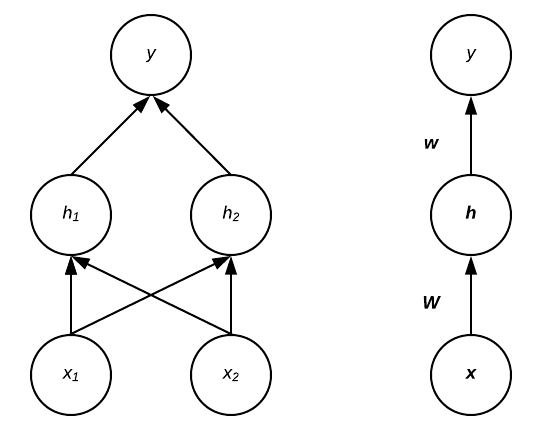
\includegraphics[scale=.5]{img/cap7_F1NN1L.png}
\end{figure}

Como se puede apreciar en la figura, los coeficientes ${\bm{W}}$ y $w$ se usan para producir el output para la siguiente capa (denominados \textbf{pesos}), por lo que la primera operaci\'on de esta red ser\'a entregar $h_{1}$ y $h_{2}$ mediante la transformaci\'on ${\bm{W}^{T}}\bm{x} + \bm{b}^{(1)}$. Luego, esta red aplica $w^{T} \boldsymbol{h} + b^{(2)}$ para producir el output $y$. Los coeficientes $\bm{b}^{(1)}$ y  $b^{(2)}$ se conocen como t\'erminos de \textbf{bias} (sesgo). Todos los parámetros de la red neuronal, los pesos y \textit{bias}, serán agrupados en el t\'ermino $\bm{\theta}$.


\subsubsection{El perceptrón y funciones de activación}

El \textit{perceptrón} corresponde a la forma más básica de una red neuronal, esta recibe un input numérico $x = (x_i)_{i=1}^n \in \R^n$ y computa la suma ponderada $u = x_1w_1 + x_2w_2 + \dots + w_nx_n + b$ donde $W = (w_i)_{i=1}^n \in \R^n$ corresponden a los \textbf{pesos} (weights) y $b \in \R$ el \textbf{sesgo} (bias). 
A continuación, se aplica una función de activación $f$ y se entrega un output $h = f(u)$.  
\begin{figure}[H]
  \centering
  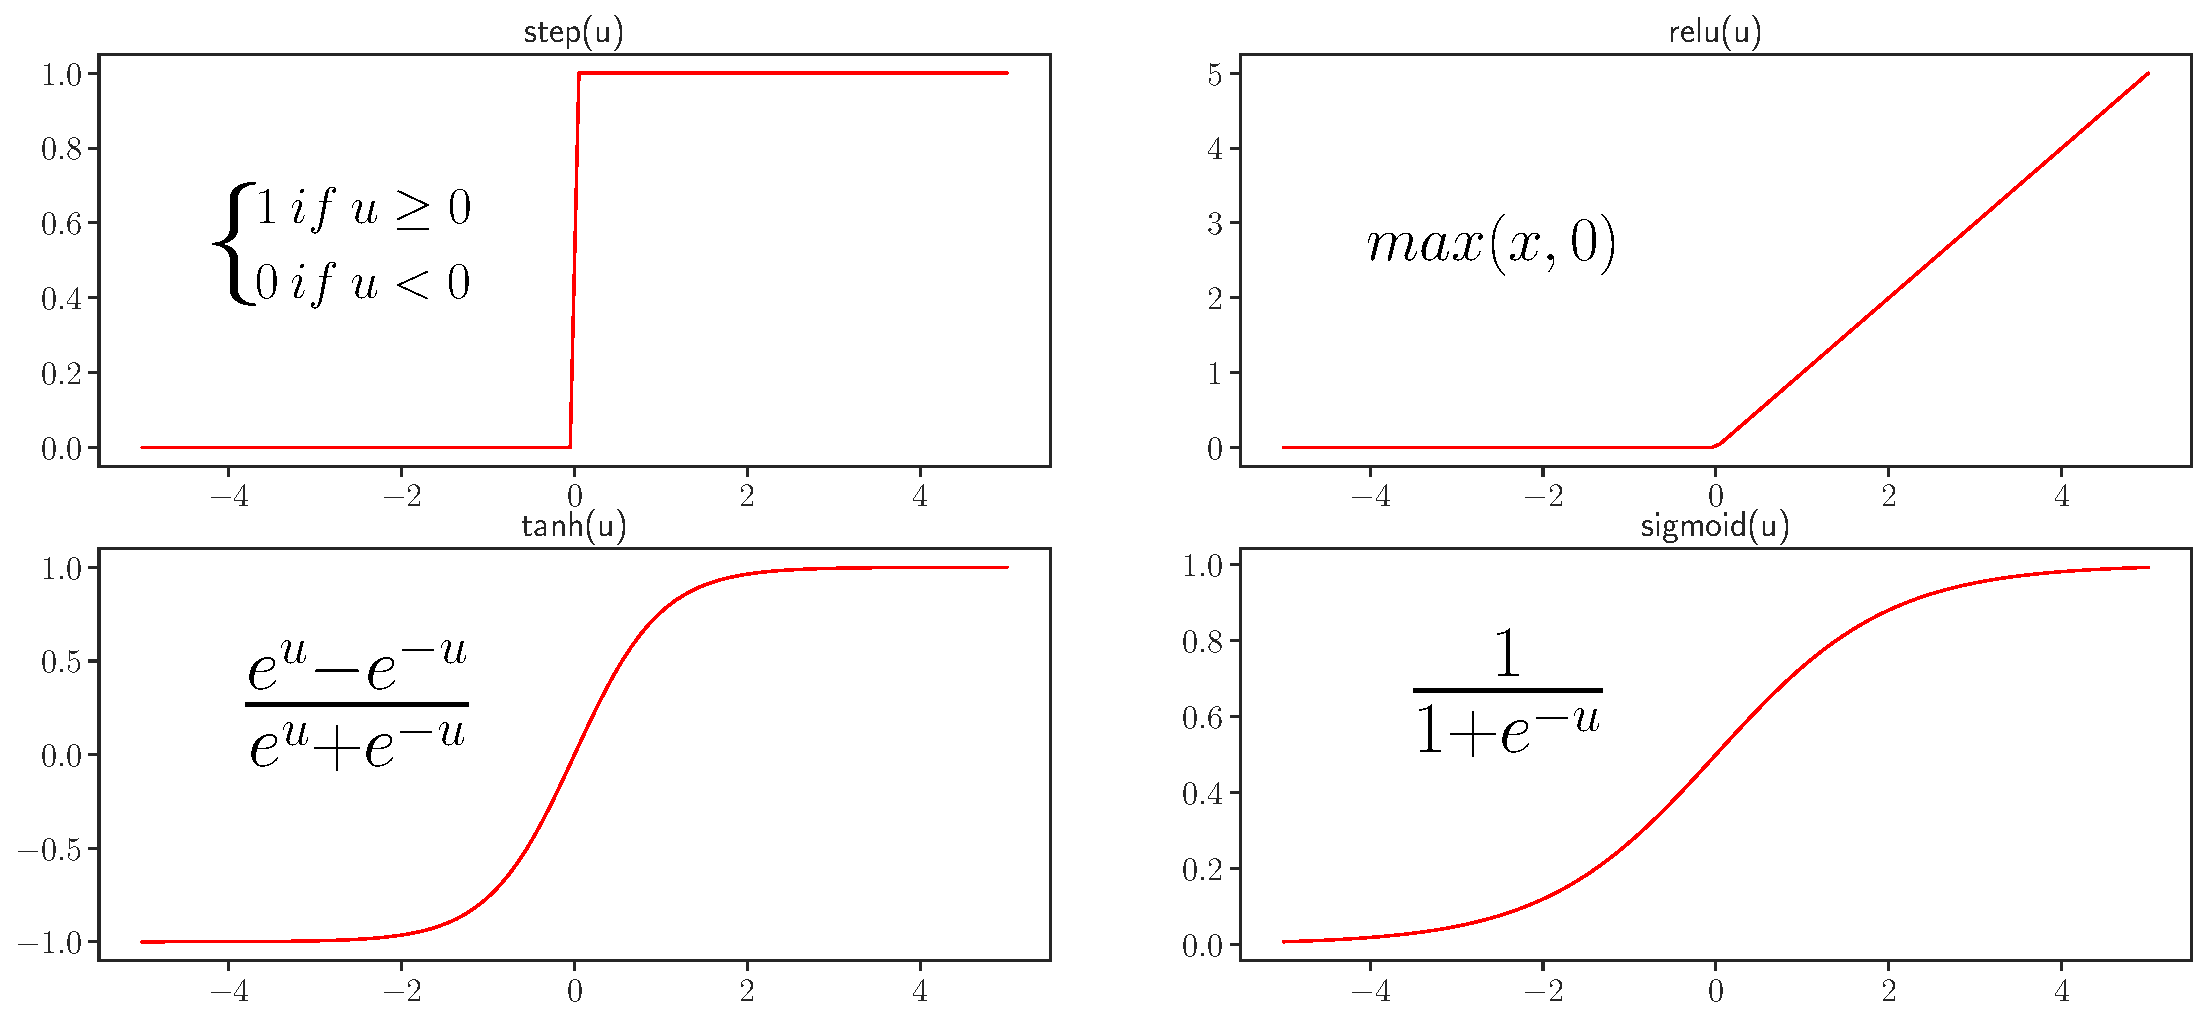
\includegraphics[scale=.3]{img/cap5_activaciones}
  \caption{Algunos ejemplos de funciones de activación}
\end{figure}

Un conjunto de perceptrones interconectados forman las capas de la red (de ahí el nombre multilayer perceptrons), las funciones de activación son en general transformaciones no lineales que buscan dar la flexibilidad necesaria al modelo para aprender funciones extremadamente complejas, lo anterior se sustenta en el siguiente teorema 


\begin{theorem}[UAT - Ancho arbitrario (Horniket al., 1989; Cybenko, 1989)]

	Sea $f^{*}$ una función objetivo Borel Medible (por ejemplo $f^{*}:[0,1]^k \rightarrow [0,1]$ continua con $k \in \N$) y sea $f$ una función de activación no polinomial acotada, entonces para todo $\epsilon > 0$ existen $W,b$ definidas como antes y $U$ la matriz de pesos de la última capa tales que 
	\[
	F(x) = f(xW+b)U, \quad 
	|F(x)-f^{*}(x)|<\epsilon \quad \forall x \in Dom(f^{*}) 
	\]
\end{theorem} 

Es decir, para una red de una sola capa escondida con la suficiente cantidad de perceptrones, es posible aproximar una función objetivo razonable tan finamente como se desee. Notar que lo anterior es un resultado que considera el ancho (cantidad de perceptrones en la capa) y que este podría ser arbitrariamente grande además, la red podría tener una baja capacidad de generalización dependiendo de la complejidad de los datos con los que se pretende trabajar. Es por esto que surge la necesidad de arquitecturas más complejas, es decir, con mayor cantidad de capas (mayor profundidad) pero menor cantidad de perceptrones y por suerte, UAT para profunidad arbitraria también es valido. 

Veamos el siguiente ejemplo: 

\begin{figure}[H]
    \centering
    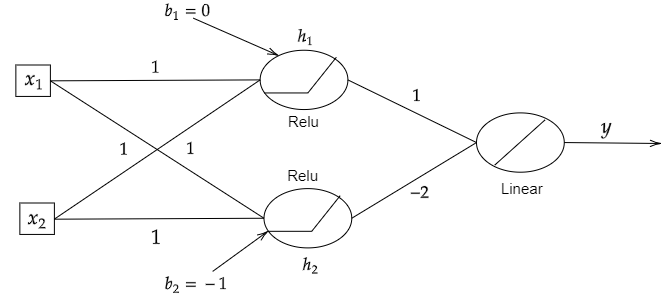
\includegraphics[scale=.5]{img/cap7_xor}
    \caption{Red Neuronal de 2 perceptrones para XOR}
\end{figure}

En su forma matricial 
$$
(h_1 , h_2) = \text{Relu} \left ( \begin{pmatrix}
x_1 & x_2  
\end{pmatrix} \begin{pmatrix}
1 &1 \\ 
 1 & 1
\end{pmatrix} + \begin{pmatrix}
0 & -1 
\end{pmatrix}\right) \hspace{0.5cm} h = \text{Relu}(xW + b)
$$

$$
y = \begin{pmatrix}
h_1 & h_2 
\end{pmatrix}\begin{pmatrix}
1 \\ 
-2 
\end{pmatrix} + (0) \hspace{0.5cm} y = hU + c
$$
Donde $U$ y $c$ corresponden al peso y bias de la última capa respectivamente, es una red capaz de computar el operador XOR.

%\begin{tabular}{| c  c | c |}
%    \hline
%    $x_1$ & $x_2$ & $y$ \\ \hline
%    0 & 0 & 0 \\
%    1 & 0 & 1 \\
%    0 & 1 & 1 \\ 
%    1 & 1 & 0 \\ \hline
%\end{tabular}. 

\subsubsection{Arquitectura de una red neuronal}

Como vimos anteriormente, no basta con una red arbitrariamente ancha para lograr el objetivo de aproximar $f^{*}$ con una alta capacidad de generalización, la \textbf{arquitectura} de una red neuronal se refiere a la totalidad de su estructura, es decir, la cantidad de capas, perceptrones por capa, conexión entre unidades, funciones de activación, etc... 

\begin{figure}[H]
	\centering
	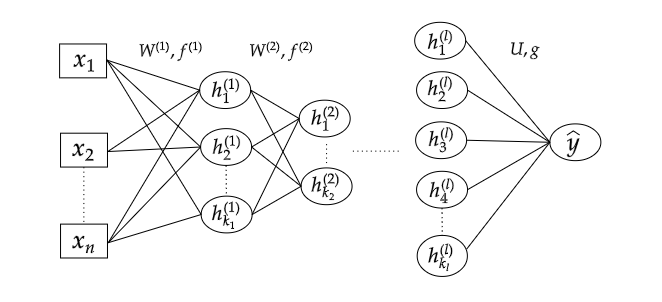
\includegraphics[scale=.5]{img/cap7_red}
	\caption{Una red con mayor profundidad}
\end{figure}

Vamos a utilizar la siguiente notación a partir de este punto 

\begin{equation}
	h^{(k)} = f^{(k)}(h^{(k-1)}W^{(k)} + b^{(k)}) \hspace{0.3cm} \forall k \in \{1 ,\dots, l\}, \quad h^{(0)}=x
	\end{equation}
	\begin{equation}
	\hat{y} = g(h^{(l)}U + c)
\end{equation}
	
Donde $g$ es la función aplicada en la capa de output y es la que define la $\textbf{unidad de output}.$

\subsubsection{Función de costos y unidades de output}

Una de las principales diferencias entre los modelos lineales antes vistos y una red neuronal, es que el uso de ciertas funciones de activaci\'on hacen que la funci\'on de costos no sea convexa, esto hace que el entrenamiento realizado en base a descenso de gradiente no entregue garant\'ias de que se alcanzar\'a el \'optimo global, o una buena solución en términos generales, ya que el algoritmo podría estancarse en un optimo local que entregue resultados pobres. 

En la mayor\'ia de los casos, el modelo param\'etrico define una distribuci\'on $p(y|\bm{x}; \bm{\theta})$, por lo que los par\'ametros del modelo se estimar\'an usando m\'axima verosimilitud, as\'i, se optimizar\'a la log-verosimilitud negativa, es decir, la \textbf{funci\'on de costos} a usar ser\'a la \textbf{cross-entropy}:

\begin{equation}
J(\bm{\theta}) = -\E_{\bm{x},\bm{y}\sim \hat{p}_{\textrm{data}}}(\textrm{log}\; p_{\textrm{modelo}}(\bm{y}|\bm{x}))
\end{equation}

De esta forma la elecci\'on de la \textbf{unidad de output} definir\'a la forma que toma la funci\'on de costos, pero no ser\'a necesario definir una funci\'on especifica para cada problema; en general siempre se resolver\'a el problema por m\'axima verosimilitud. La elecci\'on en la unidad de output depender\'a del tipo de problema que se quiera resolver, por ejemplo

\begin{enumerate}
  \item Unidad de output lineal $\hat{\bm{y}} = h^{(l)}U + c$ 

  Útil para cuando se busca retornar la media de una distribución Gaussiana condicional $p(\bm{y}|\bm{x}) = \mathcal{N}(\bm{y}|\hat{\bm{y}};\bm{I})$, el problema de maximizar la log-verosimilitud será equivalente a minimizar el error cuadrático medio por lo que resulta adecuado para un problema de regresión.

  \item Unidad de output sigmoidal $\hat{{y}} = \text{sig}(h^{(l)}U + c)$ 

  Este se utiliza para problemas de clasificación binaria, para resolver el problema de máxima verosimilitud, se modela utilizando una distribución Bernoulli en $y$ condicional en $x$. La unidad de output modela entonces $P(y=1|\bm{x})$ o la probabilidad de pertenecer a la clase 1.
   

  \item Unidad de output softmax $\hat{{y}} = \text{softmax}(h^{(l)}U + c)$  

  Es una generalización de la función sigmoidal definida como 
  \begin{equation*}
  \text{softmax}(z)_i = \frac{e^{z_i}}{\sum_{j}e^{z_j}}
  \end{equation*}
  y se utiliza para el caso de clasificación multiclase. 
  %Se podrían agregar propiedades como estabilidad numérica producto de invarianza a la adición 
\end{enumerate}


\subsection{Entrenamiento de una red neuronal}

\subsubsection{Forward Propagation}

Al usar una red neuronal \textit{feedforward}, la información fluye a través de la red desde el ingreso de un input $x$ hasta producir un output $\hat{y}$. Esto se conoce como \textbf{forward propagation} y es la que durante el entrenamiento calcula el costo $J(X, \theta)$ 
El algoritmo que la describe es el siguiente:

\begin{algorithm}[H] % H = forzar está posición 
	\caption{Forward Propagation}\label{ML:Algorithm1}
	\textbf{Requerir}: Profundidad de la red, $l$ \\
	\textbf{Requerir}: $\bm{W}^{(k)}, k \in \{1,...,l\}$, pesos de la red \\
	\textbf{Requerir}: $\bm{b}^{(k)}, k \in \{1,...,l\}$, parámetros bias de la red \\
	\textbf{Requerir}: $\bm{x}$, el input \\
	\textbf{Requerir}: $U,c,g$, matriz de peso, bias y función de output de la última capa respectivamente 
	\begin{algorithmic}[1]
		\State $\bm{h}^{(0)} \gets \bm{x}$
		\For{$\;k = 1,...,l$:}
			\State $\bm{u}^{(k)} \gets  \bm{h}^{(k-1)}\bm{W}^{(k)} + \bm{b}^{(k)}$
			\State $\bm{h}^{(k)} \gets f^{(k)}(\bm{u}^{(k)})$
		\EndFor
		\State $\bm{\hat{y}} \gets g(\bm{h}^{(l)}U+c)$
		\State $J \gets L(\bm{\hat{y}},\bm{y})$
	\end{algorithmic}

\end{algorithm}


\subsubsection{Backward Propagation - Preliminares}

El algoritmo de $\textbf{backpropagation}$ permite que la información del costo fluya en sentido inverso a través de la red para calcular el gradiente de manera computacionalmente eficiente. 

El gradiente se calculará de esta forma ya que, aunque es posible obtener una expresión analítica para este, evaluar la expresión puede ser muy caro computacionalmente. 

Luego de obtener el gradiente, otro algoritmo como descenso de gradiente estocástico realizará el aprendizaje usando la expresión que fue calculada. 

El algoritmo de backpropagation ha experimentatdo un resurgimiento en estas últimas décadas por su implementación en redes neuronales para tareas tales como reconocimiento de imágenes o procesamiento de lenguaje natural. 
Es considerado un algoritmo eficiente e implementaciones modernas de estas aprovechan el paralelismo de las GPU para mejorar su rendimiento. 

Antes de comenzar a describir el algoritmo, debemos tener en cuenta que.   
\begin{itemize}

	\item Utilizaremos la notación para el paso intermedio antes de aplicar la función de activación como $u = hW + b$
  
	\item Es recurrente que en la etapa de entrenamiento de la red el conjunto de datos se entreguen en pequeños paquetes (\textbf{mini-batch}), es decir $(x^d)_{d=1}^N$  conjunto de $N$ inputs, luego $u_{dj}^{(k)}$ corresponde al valor de $u$ para el input $d$ en el nodo $j$ para la capa $k$. Todo esto con el fin de aprovechar lo más posible la optimización en operaciones de matrices que ofrecen las GPU.

   
   \item Haremos la deducción del algoritmo de backpropagation para una función de error MSE en un problema de regresión.
   \[
	J(X ,\theta) = \frac{1}{2N}\sum_{d=1}^N(\hat{y}_d-y_d)^2
	\]	
  
\end{itemize} 

Nuestro objetivo será actualizar todos los valores $w_{ij}^{(k)}$ (peso del nodo $i$ al nodo $j$ en la capa $k$). Es decir, para utilizar el método del descenso de gradiente es necesario calcular $\frac{\partial J(X , \theta) }{\partial w_{ij}^{(k)}}$ notemos que 
\[
\frac{\partial J(X , \theta) }{\partial w_{ij}^{(k)}} = \frac{1}{N}\sum_{d=1}^N \frac{\partial}{\partial w_{ij}^{(k)}} \left ( \frac{1}{2}(\hat{y}_d-y_d)^2 \right) = \frac{1}{N}\sum_{i=1}^N \frac{\partial J_d}{\partial w_{ij}^{(k)}}
\]

Utilizando la regla de la cadena 
\[
\frac{\partial J_d}{\partial w_{ij}^{(k)}} = \frac{\partial J_d}{\partial u_{dj}^{(k)}}\frac{\partial u_{dj}^{(k)}}{\partial w_{ij}^{(k)}}
\] 
La expresión $\frac{\partial J_d}{\partial u_{dj}^{(k)}}$ corresponde a un término de \textbf{error} y lo denotaremos \
\[
\delta_{dj}^{(k)} \equiv \frac{\partial J_d}{\partial u_{dj}^{(k)}}
\] 
Mientras que para el otro término tenemos que 
\[
\frac{\partial u_{dj}^{(k)}}{\partial w_{ij}^{(k)}} = \frac{\partial}{\partial w_{ij}^{(k)}} \left ( \sum_{a = 1}^{k_k}w_{aj}^{(k)}h_{da}^{(k-1)} + b_j^{(k)} \right) = h_{di}^{(k-1)}
\] 
y así 
\[
\frac{\partial J_d}{\partial w_{ij}^{(k)}} = \delta_{dj}^{(k)}  h_{di}^{(k-1)}
\]
El gradiente total, será la suma de los $N$ gradientes y que expresaremos en su forma matricial
\begin{equation}
\frac{\partial J}{\partial w_{ij}^{(k)}} = \sum_{d=1}^N \delta_{dj}^{(k)}  h_{di}^{(k-1)}  \Rightarrow  \frac{\partial J}{\partial W^{(k)}} = (h^{(k-1)})^T @ \hspace{0.1cm} \delta^{(k)}
\end{equation}
Omitiremos la constante $1/N$ hasta el final del algoritmo.




\subsubsection{Backward Propagation - Capas ocultas}

Nuevamente, de la regla de la cadena
\[
\delta_{dj}^{(k)} = \frac{\partial J_d}{\partial u_{dj}^{(k)}} = \sum_{a=1}^{k_{k+1}} \frac{\partial J_d}{\partial u_{da}^{(k+1)}} \frac{\partial u_{da}^{(k+1)}}{\partial u_{dj}^{(k)}} = \sum_{a=1}^{k_{k+1}} \delta_{da}^{(k+1)} \frac{\partial u_{da}^{(k+1)}}{\partial u_{dj}^{(k)}}
\] 

no es difícil ver que

\[
\frac{\partial u_{da}^{(k+1)}}{\partial u_{dj}^{(k)}} = w_{ja}^{(k+1)}f'(u_{dj}^{(k)})  \Rightarrow  \delta_{dj}^{(k)} = f'(u_{dj}^{(k)})\sum_{a=1}^{k_{k+1}}w_{ja}^{(k+1)}\delta_{da}^{(k+1)}
\]

Hemos encontrado una expresión para calcular el gradiente en una capa $k$ en base al gradiente de la siguiente capa $k+1$ (De aquí el nombre \textbf{backward propagation}).
\newline 

Lo anterior en su forma matricial queda descrito por
\begin{equation}
\delta^{(k)} = f'(u^{(k)}) * \left ( \delta^{(k+1)} @ \hspace{0.1cm} (W^{(k+1)})^T \right )
\end{equation}
Lo único que queda para presentar el algoritmo final es calcular los gradientes en la última capa (output)


\subsubsection{Backward Propagation - Capa de output}

Estamos suponiendo un problema de regresión por lo que el output será de una sola salida y la función de error es MSE, entonces 
\[
\delta_{d1}^{(l)} = \frac{\partial J_d}{\partial u_{d1}^{(l)}} = (\hat{y}_d-y_d) (\hat{y}_d)' 
\] 
Además, la función de activación en el output será lineal y por tanto $(\hat{y}_d)' = 1$, finalmente el término de normalización $N$ se agrega en este paso.  La forma matricial queda en 
\begin{equation}
\label{eq:capa_output}
\delta_{1}^{(l)} = \frac{1}{N}(\hat{y}-y)
\end{equation}

\begin{algorithm}[H]
	\caption{Backward Propagation - Regresión} \label{ML:Algorithm2}
	\textbf{Requerir: } learning rate $\lambda$ para descenso de gradiente estocástico
	\begin{algorithmic}[1]
	\State Forward propagation, guardar  ($\hat{y})_d$ , $(u_{ij}^{(k)})_{ijd}$ y $(h_{ij}^{(k)})_{ijd}$.
	\State Evaluar el error de la última capa $\delta_1^{(l)}$  utilizando las ecuaciones en la capa de output 
	\For{$k = 1,...,l-1$:}
		\For{$i,j$}
			\State Propagar hacia atrás y calcular el error $\delta^{(k)}$ de las ecuaciones en la capa oculta 
			\State Evaluar las derivadas parciales $\frac{\partial J}{\partial w_{ij}^{(k)}}$ y $\frac{\partial J}{\partial b_j^{(k)}}$
			\State Actualizar $w_{ij}^{(k)} \gets w_{ij}^{(k)} - \lambda \frac{\partial J}{\partial w_{ij}^{(k)}}$
			\State Actualizar $b_{j}^{(k)} \gets b_{j}^{(k)} - \lambda \frac{\partial J}{\partial b_{j}^{(k)}}, \quad$
		\EndFor
	\EndFor

	\end{algorithmic}
	
\end{algorithm}

\begin{remark}
	El algoritmo anterior fue descrito para cada uno de los pesos $w_{ij}^{(k)}$ y bias $b_{j}^{(k)}$ pero en la práctica, se utilizan operaciones matriciales para actualizar los pesos en las capas.
\end{remark}

\begin{remark}
	El algoritmo anterior debe ser aplicado para todos los batch del conjunto de entrenamiento, la cantidad de veces que se pase por todos los datos de entrenamiento, se conoce como \textbf{épocas}, en general un mayor número de épocas disminuye el error de entrenamiento, sin embargo, muchas épocas podrían reducir la capacidad de generalización debido al \textbf{overfitting}.	
\end{remark}

\section{Regularización}










